101. \begin{figure}[ht!]
\center{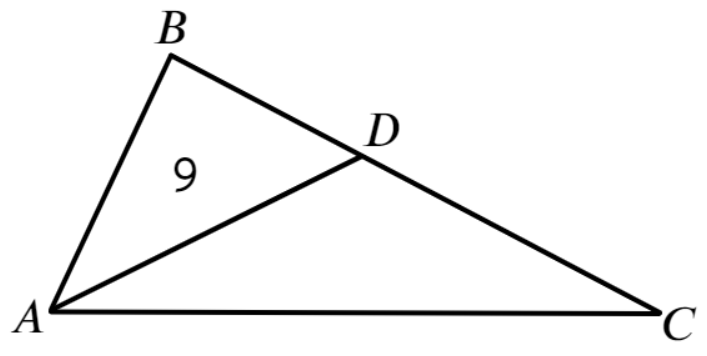
\includegraphics[scale=0.35]{g9-101.png}}
\end{figure}\\
По свойству основания биссектрисы имеем равенство $\cfrac{BD}{DC}=\cfrac{AB}{AC}=\cfrac{3}{5}.$ У треугольников $ABD$ и $ACD$ общая высота из точки $A,$ значит $\cfrac{S_{\Delta ABD}}{S_{\Delta ACD}}=\cfrac{BD}{DC}=\cfrac{3}{5},\ S_{\Delta ACD}=9\cdot\cfrac{5}{3}=15\text{ см}^2.$\\
